
\chapter{Characterization of the Human Body Lower Limb} \label{appendixA}
\section{Stacked Clustered Bar Charts}
This appendix presents the compiled data from the reviewed gait analysis studies, in the form of charts as the ones presented in \Cref{sec:characterizationKKP}, for the hip, knee and ankle joints. The parameters of torque, angle and power, are extracted.

\begin{figure}[htbp]
\centering
    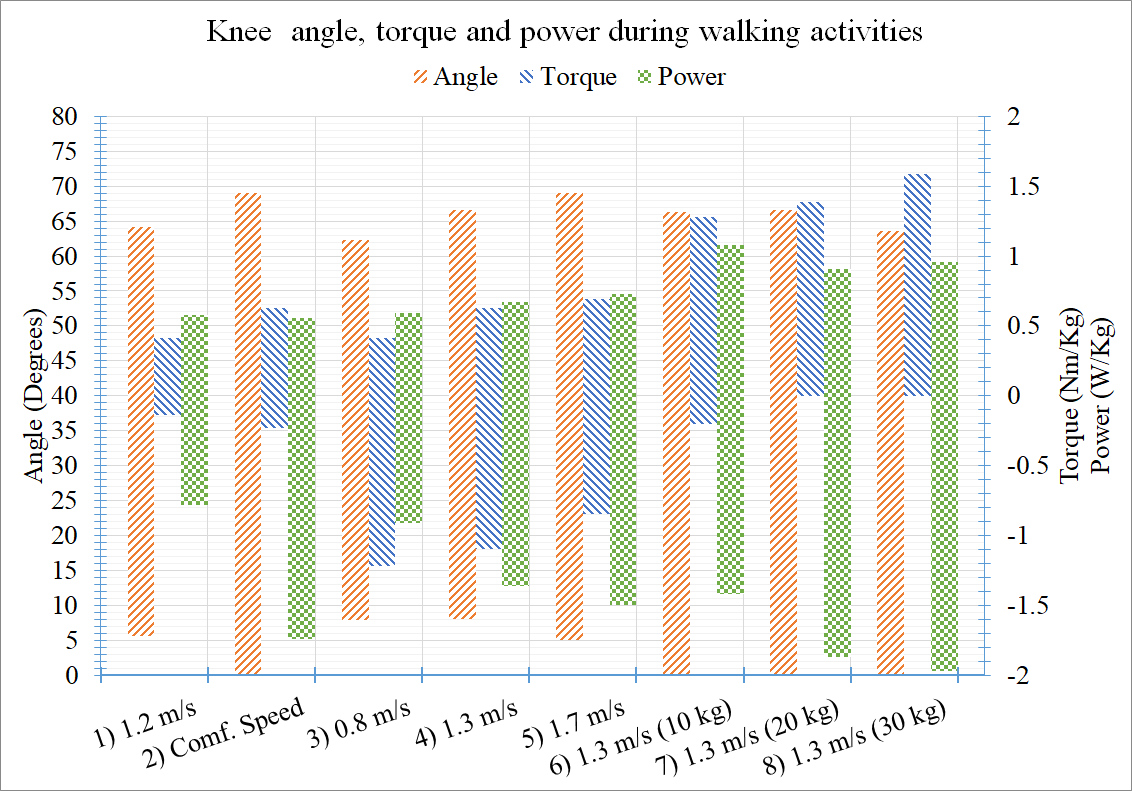
\includegraphics[width=\textwidth]{KneeKKPWalkingExcel.png}
    \caption[Knee joint characteristics for walking over ground activities. The weight next to the name of some activities dictates the load carried by the subjects during the experiment.]{Knee joint characteristics for walking over ground activities. The weight next to the name of some activities dictates the load carried by the subjects during the experiment \cite{solis2017characterization}. Data collected from: (1) \cite{bovi2011multiple}, (2) \cite{lee2008biomechanics}, (3-8) \cite{han2011biomechanical}.}
    \label{fig:kneeKKPWalking}
\end{figure}

\begin{figure}[htbp]
\centering
    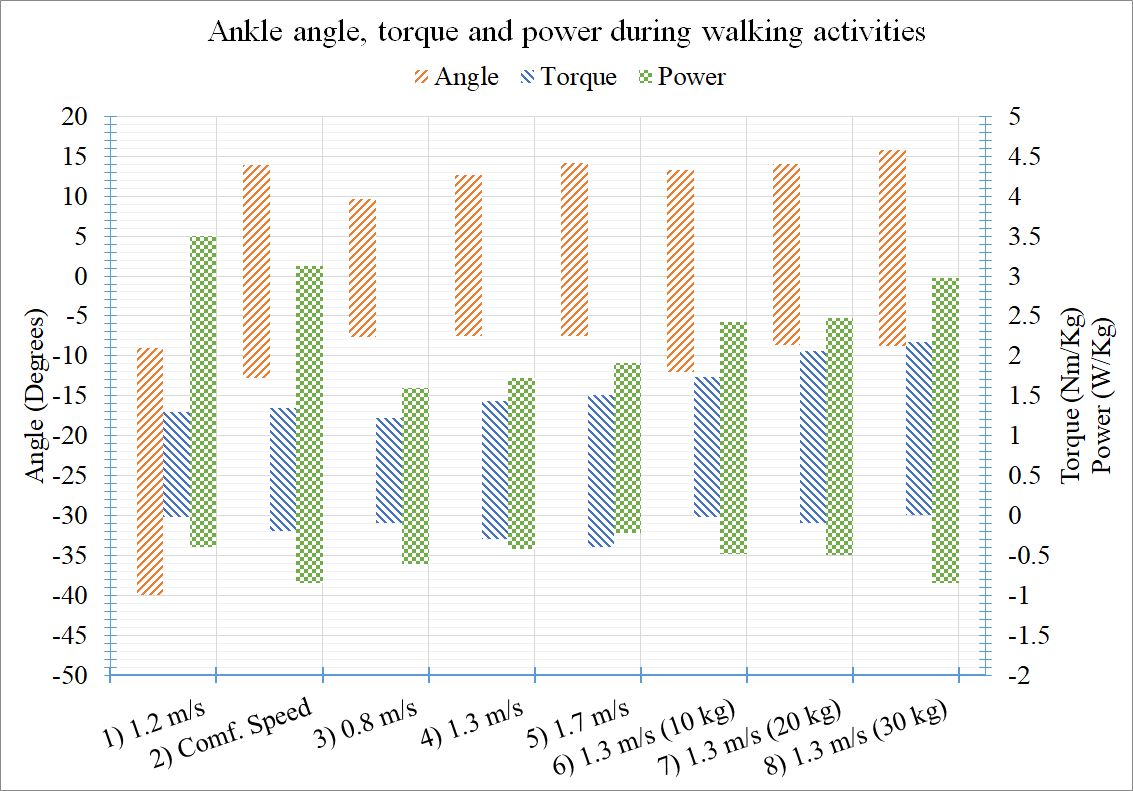
\includegraphics[width=0.9\textwidth]{AnkleKKPWalkingExcel.png}
    \caption[Ankle joint characteristics for walking over ground activities. The weight next to the name of some activities dictates the load carried by the subjects during the experiment.]{Ankle joint characteristics for walking over ground activities. The weight next to the name of some activities dictates the load carried by the subjects during the experiment \cite{solis2017characterization}. Data collected from: (1) \cite{bovi2011multiple}, (2) \cite{lee2008biomechanics}, (3-8) \cite{han2011biomechanical}.}
    \label{fig:ankleKKPWalking}
\end{figure}

\begin{figure}[htbp]
    \centering
    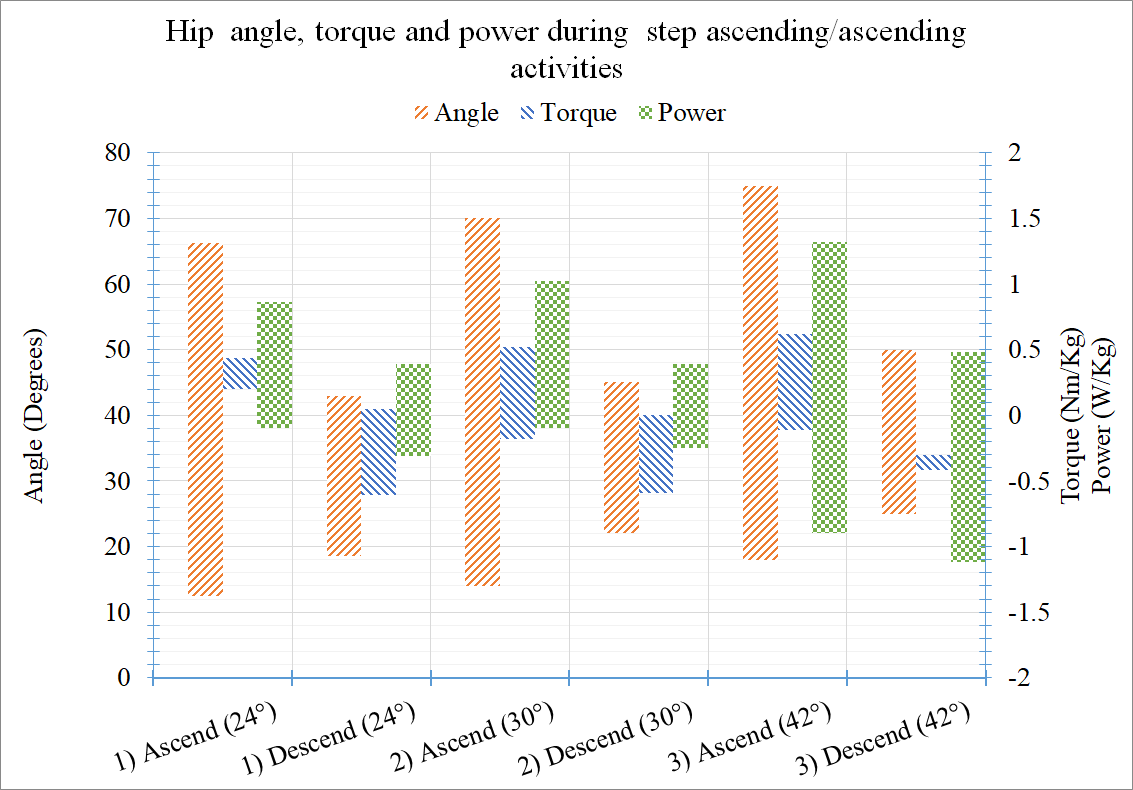
\includegraphics[width=0.9\textwidth]{HipKKPStairsExcel.png}
    \caption[Hip joint characteristics for step ascending/descending experiments.]{Hip joint characteristics for step ascending/descending experiments \cite{solis2017characterization}. Data collected from: (1) \cite{protopapadaki2007hip}, (2) \cite{riener2002stair}, (3) \cite{reid2007knee}. }
    \label{fig:hipKKPStairs}
\end{figure}

\begin{figure}[htbp]
    \centering
    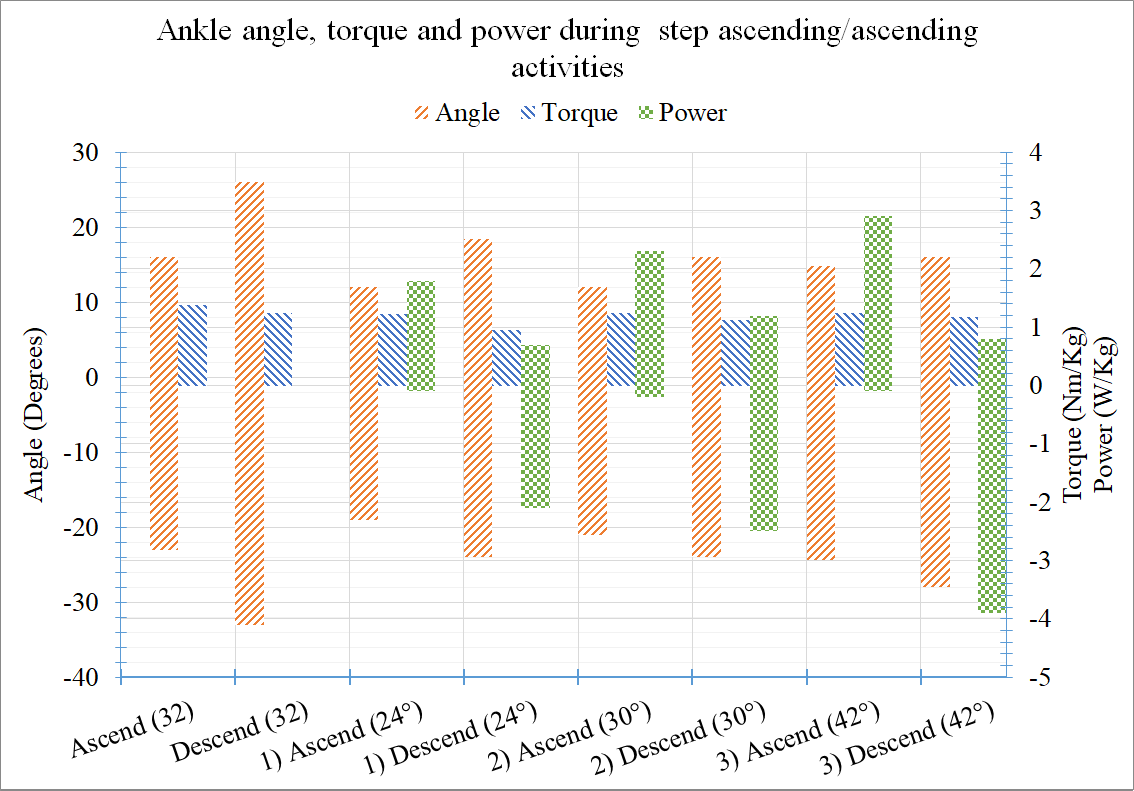
\includegraphics[width=0.9\textwidth]{AnkleKKPStairsExcel.png}
    \caption[Ankle joint characteristics for step ascending/descending experiments.]{Ankle joint characteristics for step ascending/descending experiments \cite{solis2017characterization}. Data collected from: (1) \cite{protopapadaki2007hip}, (2) \cite{riener2002stair}, (3) \cite{reid2007knee}. }
    \label{fig:ankleKKPStairs}
\end{figure}

\begin{figure}[htbp]
    \centering
    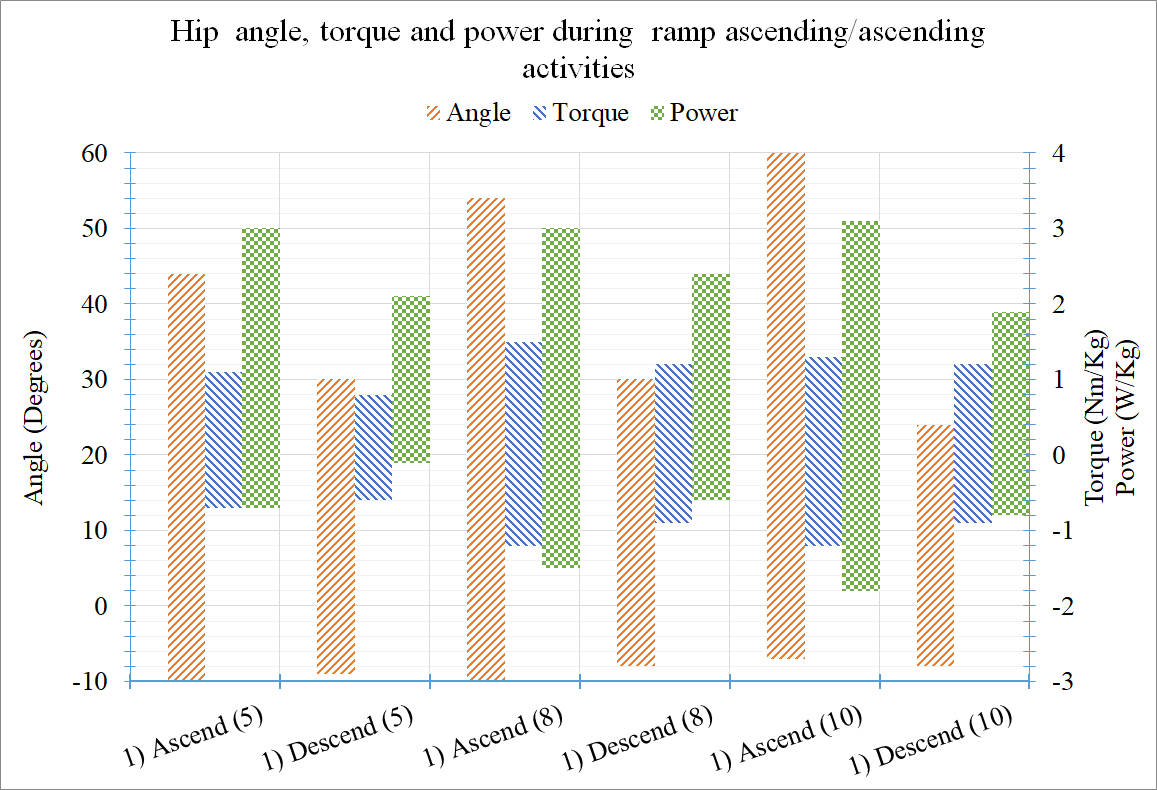
\includegraphics[width=0.9\textwidth]{HipKKPRampExcel.png}
    \caption[Hip joint characteristics for ramp ascending/descending experiments. Inclination in brackets.]{Hip joint characteristics for ramp ascending/descending experiments \cite{solis2017characterization}. Inclination in brackets. Data collected from \cite{mcintosh2006gait}}
    \label{fig:hipKKPRamp}
\end{figure}

\begin{figure}[htbp]
    \centering
    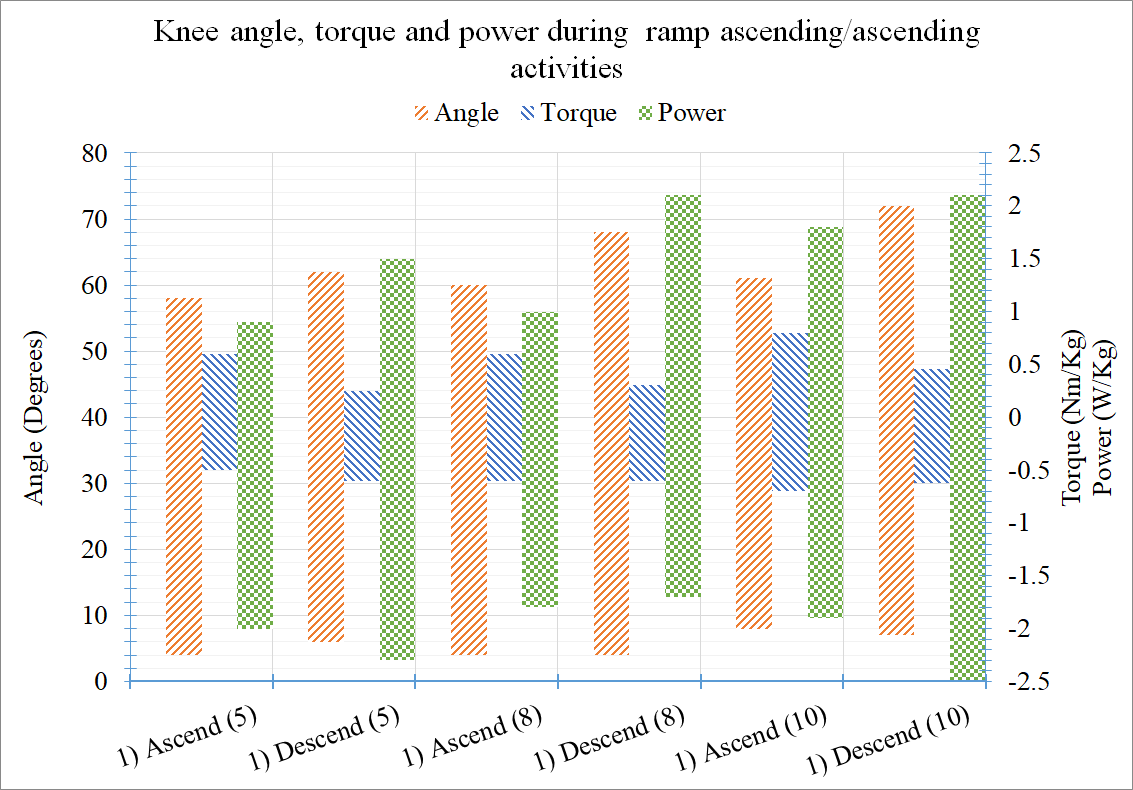
\includegraphics[width=0.9\textwidth]{KneeKKPRampExcel.png}
    \caption[Knee joint characteristics for ramp ascending/descending experiments. Inclination in brackets.]{Knee joint characteristics for ramp ascending/descending experiments \cite{solis2017characterization}. Inclination in brackets. Data collected from \cite{mcintosh2006gait}. }
    \label{fig:kneeKKPRamp}
\end{figure}

\begin{figure}[htbp]
    \centering
    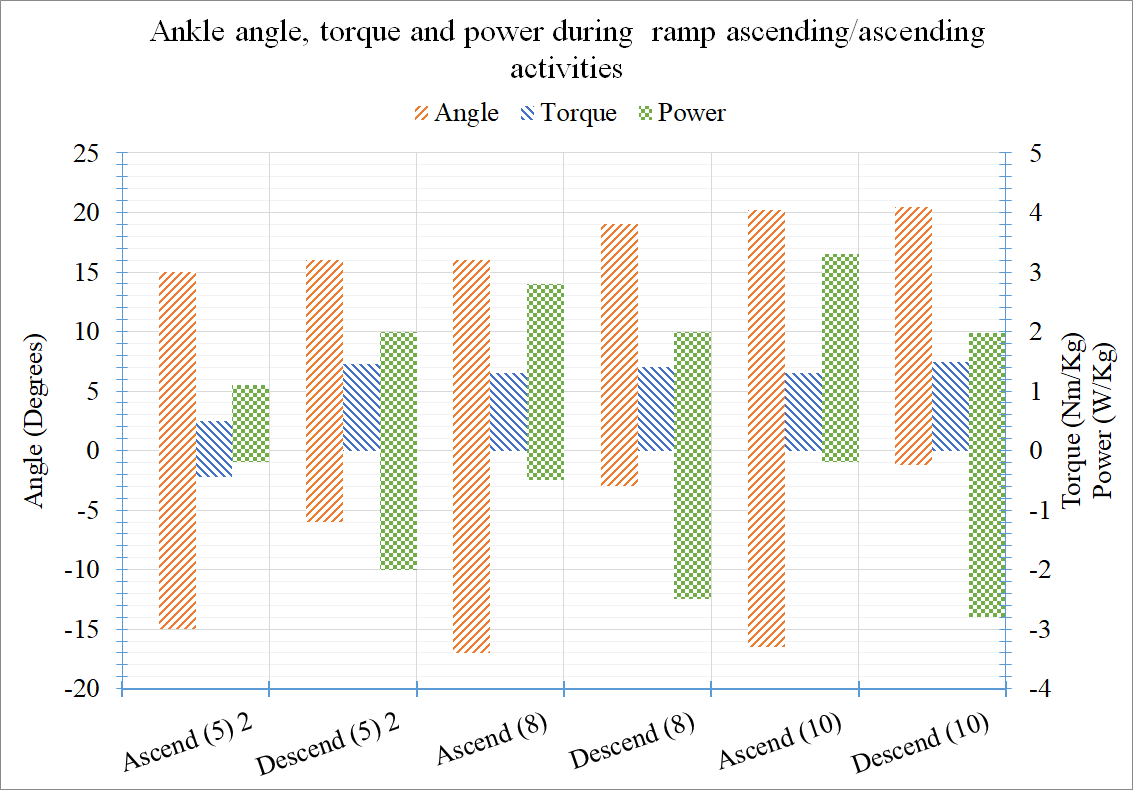
\includegraphics[width=0.8\textwidth]{AnkleKKPRampExcel.png}
    \caption[Ankle joint characteristics for ramp ascending/descending experiments. Inclination in brackets.]{Ankle joint characteristics for ramp ascending/descending experiments \cite{solis2017characterization}. Inclination in brackets. Data collected from \cite{mcintosh2006gait}.}
    \label{fig:ankleKKPRamp}
\end{figure}

\begin{figure}[htbp]
    \centering
    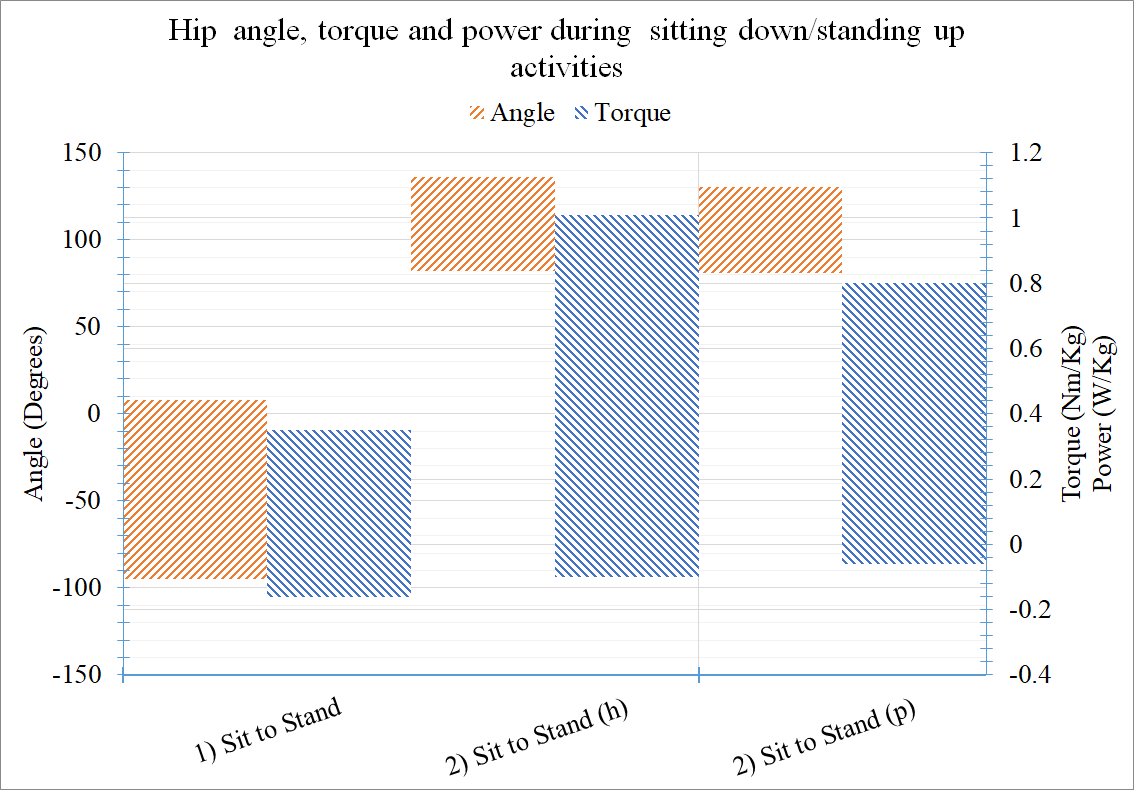
\includegraphics[width=0.8\textwidth]{HipKKPSitExcel.png}
    \caption[Hip joint characteristics for sit to stand/stand to sit experiments. In brackets (h) healthy subjects, and (p) subjects with Parkinson's.]{Hip joint characteristics for sit to stand/stand to sit experiments \cite{solis2017characterization}. In brackets (h) healthy subjects, and (p) subjects with Parkinson's. Data collected from: (1) \cite{roebroeck1994biomechanics}, (2) \cite{mak2003joint}.  }
    \label{fig:hipKKPSit}
\end{figure}

\begin{figure}[htbp]
    \centering
    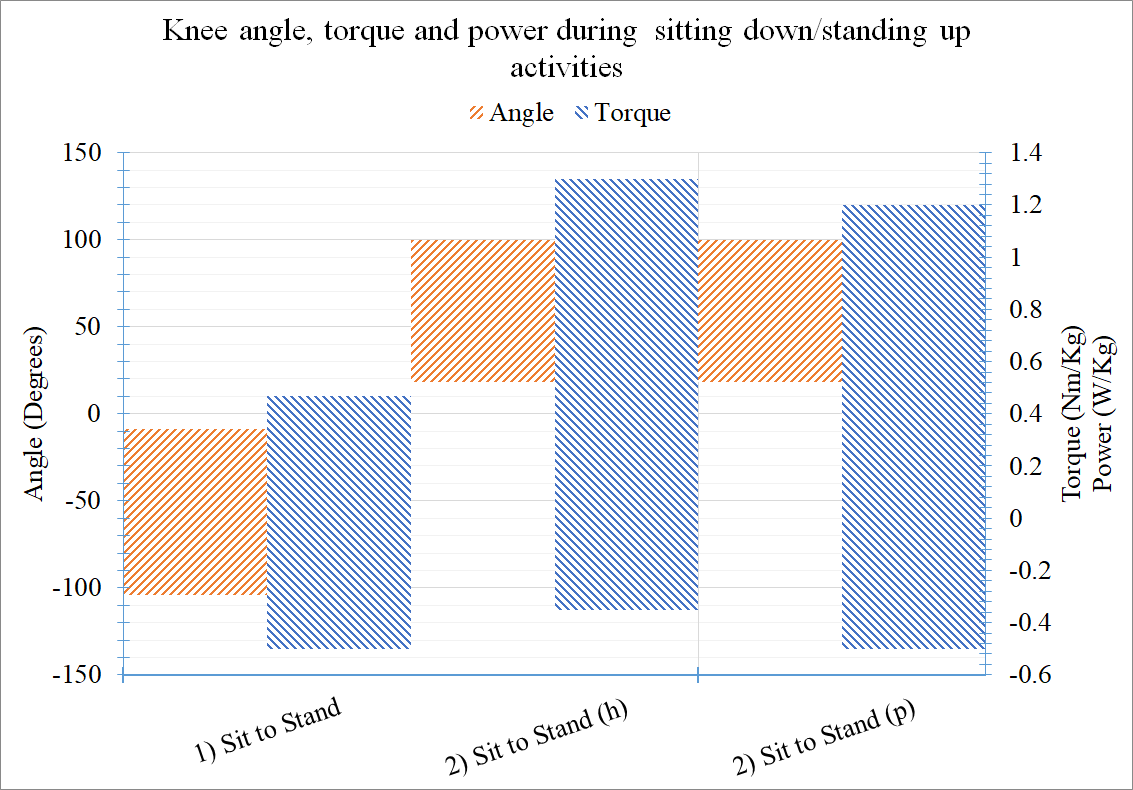
\includegraphics[width=0.8\textwidth]{KneeKKPSitExcel.png}
    \caption[Knee joint characteristics for sit to stand/stand to sit experiments. In brackets (h) healthy subjects, and (p) subjects with Parkinson's.]{Knee joint characteristics for sit to stand/stand to sit experiments \cite{solis2017characterization}. In brackets (h) healthy subjects, and (p) subjects with Parkinson's. Data collected from: (1) \cite{roebroeck1994biomechanics}, (2) \cite{mak2003joint}.  }
    \label{fig:kneeKKPSit}
\end{figure}

\begin{figure}[htbp]
    \centering
    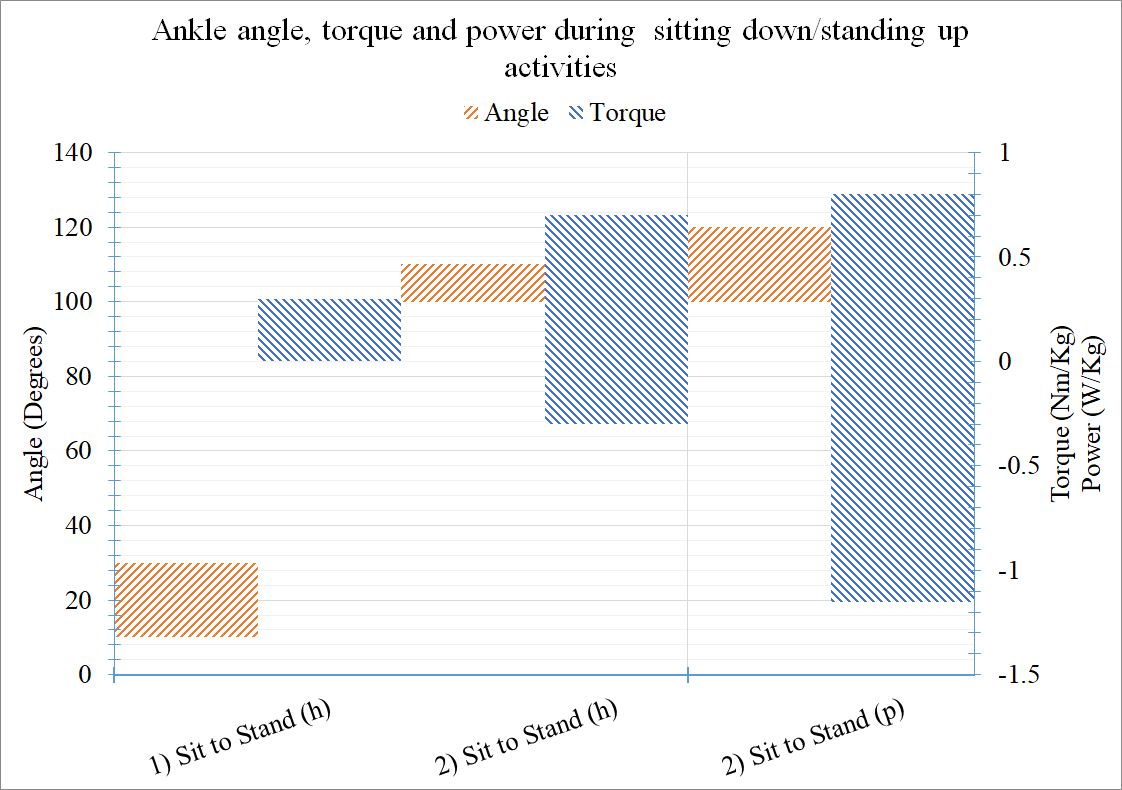
\includegraphics[width=\textwidth]{AnkleKKPSitExcel.png}
    \caption[Ankle joint characteristics for sit to stand/stand to sit experiments. In brackets (h) healthy subjects, and (p) subjects with Parkinson's.]{Ankle joint characteristics for sit to stand/stand to sit experiments \cite{solis2017characterization}. In brackets (h) healthy subjects, and (p) subjects with Parkinson's. Data collected from: (1) \cite{roebroeck1994biomechanics}, (2) \cite{mak2003joint}.  }
    \label{fig:ankleKKPSit}
\end{figure}

